\chapter{Empirical Analysis}

\textit{``\textendash\ Those dying generations \textendash\ at their song,\\
The salmon-falls, the mackerel-crowded seas,\\
Fish, flesh, or fowl, commend all summer long\\
Whatever is begotten, born, and dies''.\\
\textemdash\ ``Sailing to Byzantium'' by William Butler Yeats }

\vspace{.2cm}

\section{Regression Results Summary}

Firstly is the formula of GAM and FAD LM:
\vspace{-14pt}
\begin{align*}
\texttt{E(popgap)} = & - 7.420 - 0.079 \times \texttt{potato\_price} + f_1(\texttt{grain\_price\_other}) \\
                & + 0.342 \times \texttt{ground\_rent} + \textcolor{red}{0.45 \times \texttt{factor(if\_tithe)}} \\
                & + f_2(\texttt{general\_wage})  \\
                & + 0.044 \times \texttt{imports\_total} + \textcolor{red}{f_3(\texttt{exports\_total})}\\
                & + 3.616 \times \texttt{factor(poorlaw)} \\
                & + \epsilon \\
\texttt{popgap} = & \ 1.987 - 0.003 \times \texttt{grain\_acre\_total} + \epsilon
\end{align*}

The non-significant items have been highlighted in red. All hypotheses are significant for at least one variable, thus allowing for further coefficient interpretation. Table 5.1 lists the values and significance of the coefficients to facilitate comparisons between the model and the hypotheses.

In terms of the trade-based entitlement, an 1 unit increase in the price of potatoes, the population change within a year is associated with an average increase of -7\%; In terms of the production-based entitlement, an 1 unit increase in the ground rent, the population change within a year is associated with an average increase of 34\%; In terms of the inheritance and transfer entitlement, an 1 unit increase in the grain imports, the population change within a year is associated with an average increase of 4\% also the year with poor law will have an average 36\% increase in population change compared with year without poor law.

\begin{table}[h]
    \centering
    \caption{GAM, FAD LM, and General LM}
    \begin{tabular}{@{\extracolsep{5pt}}lccc}
    \\[-1.8ex]\hline
    \hline \\[-1.8ex]
    & \multicolumn{3}{c}{\textit{Dependent variable: popgap}} \\
    \cline{2-4}
    \\[-1.8ex] & GAM & FAD LM & General LM \\
    \hline \\[-1.8ex]
    potato\_price & $-$0.079$^{***}$ & & $-$0.107$^{***}$ \\
     & (0.028) & & (0.033) \\
    grain\_price\_other & &  & 0.179$^{**}$ \\
     & &  & (0.069) \\
    grain\_acre\_total & & $-$0.003$^{***}$ & \\
     & & (0.001) & \\
    ground\_rent & 0.342$^{***}$ & & 0.082 \\
     & (0.118) & & (0.119) \\
    factor(if\_tithe)1 & 0.450 & & 1.159$^{**}$ \\
     & (0.559) & & (0.535) \\
    general\_wage & & & 0.050 \\
     & & & (0.037) \\
    imports\_total & 0.044$^{***}$ & & 0.042$^{***}$ \\
     & (0.008) & & (0.010) \\
    exports\_total & & & 0.001 \\
     & & & (0.001) \\
    factor(poorlaw)1 & 3.616$^{***}$ & & 3.103$^{***}$ \\
     & (0.617) & & (0.752) \\
    Constant & $-$7.420$^{***}$ & 1.987$^{**}$ & $-$7.751$^{***}$ \\
     & (1.391) & (0.796) & (1.964) \\
    \hline \\[-1.8ex]
    s(grain\_price\_other) & $^{**}$ & & \\
    s(general\_wage) & $^{***}$ & & \\
    s(exports\_total) &  & & \\
    \hline \\[-1.8ex]
    Observations & 80 & 80 & 80 \\
    Adjusted R$^{2}$ & 0.741 & 0.097 & 0.570 \\
    AIC & 201.470 & & 235.916 \\
    Residual Std. Error & & 1.436 (df = 78) & 0.990 (df = 71) \\
    F Statistic & & 9.457$^{***}$ (df = 1; 78) & 14.115$^{***}$ (df = 8; 71) \\
    \hline
    \hline \\[-1.8ex]
    \textit{Note:}  & \multicolumn{3}{r}{$^{*}$p$<$0.1; $^{**}$p$<$0.05; $^{***}$p$<$0.01} \\
    \end{tabular}
\end{table}

In addition to the regular terms, the smoothed terms are equally important in the GAM. The visualization of significant smoothing term is shown in Figure 5.1.

\begin{figure}[h]
    \centering
    \caption{Significant Smooth Term Plot}
    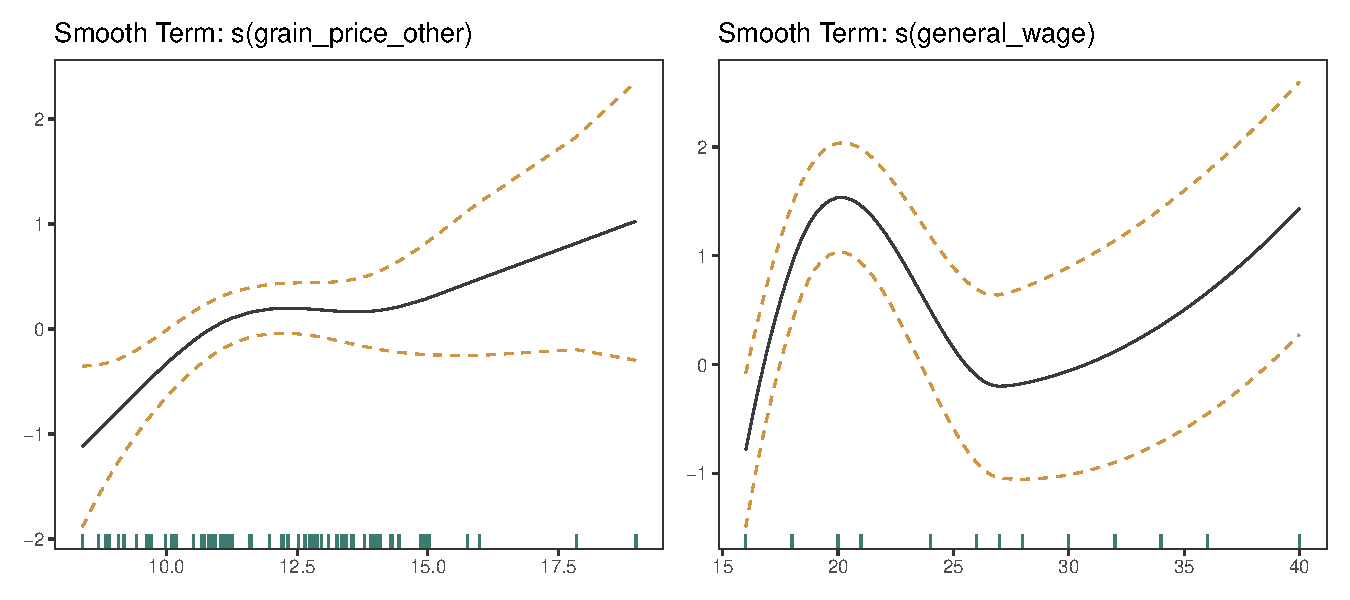
\includegraphics[width=.95\textwidth]{../03_outputs/smoothterm.pdf}
\end{figure}

\section{Robustness Test}

\begin{table}[h]
    \centering
    \caption{Regression Model Comparisons}
    \begin{tabular}{@{\extracolsep{5pt}}lccccc}
    \\[-1.8ex]\hline
    \hline \\[-1.8ex]
    & \multicolumn{5}{c}{\textit{Dependent variable: popgap}} \\
    \cline{2-6}
    \\[-1.8ex] & GAM 1 & LM & GAM 2 & GAM 3 & GAM 4 \\
    & \textit{standard} & \textit{linear} & \textit{year} & \textit{half year} & \textit{dif.} \\
    \hline \\[-1.8ex]
    potato\_price & $-$0.079$^{***}$ & $-$0.107$^{***}$ & $-$0.096$^{**}$ & $-$0.133$^{**}$ & $-$0.063$^{*}$ \\
     & (0.028) & (0.033) & (0.028) & (0.050) & (0.025) \\
    grain\_price\_other & & 0.178$^{*}$ &  & & \\
     & & (0.069) &  & & \\
    ground\_rent & 0.342$^{***}$ & 0.082 & 0.306$^{*}$ & 0.266$^{.}$ & 0.323$^{**}$ \\
     & (0.118) & (0.119) & (0.123) & (0.155) & (0.111) \\
    factor(if\_tithe)1 & 0.450 & 1.159$^{*}$ & 0.905 & 1.999$^{.}$ & 0.924$^{.}$ \\
     & (0.559) & (0.535) & (0.610) & (1.086) & (0.509) \\
    general\_wage & & 0.050 & & 1.021$^{***}$ & 1.021$^{***}$ \\
     & & (0.037) & & (0.261) & (0.261) \\
    imports\_total & 0.044$^{***}$ & 0.042$^{***}$ & 0.032$^{***}$ & 0.049$^{***}$ & 0.056$^{***}$ \\
     & (0.008) & (0.010) & (0.009) & (0.012) & (0.008) \\
    exports\_total & & 0.001 & & & \\
     & & (0.001) & & & \\
    factor(poorlaw)1 & 3.616$^{***}$ & 3.103$^{***}$ & 2.867$^{***}$ & 3.832$^{***}$ & 3.812$^{***}$ \\
     & (0.617) & (0.752) & (0.664) & (0.901) & (0.523) \\
    \hline \\[-1.8ex]
    s(grain\_price\_other) & $^{**}$ & & $^{**}$ & $^{*}$ & $^{***}$  \\
    s(general\_wage) & $^{***}$ & & $^{***}$ & & $^{***}$ \\
    s(exports\_total) & & & \\
    \hline \\[-1.8ex]
    Observations & 80 & 80 & 80 & 40 & 80 \\
    \hline
    \hline \\[-1.8ex]
    \textit{Note:} & \multicolumn{5}{r}{$^{*}$p$<$0.1; $^{**}$p$<$0.05; $^{***}$p$<$0.01} \\
    \end{tabular}
\end{table}
